\input preamble.tex
\noindent
\section*{Industrielektronikk Øving 05 - Serie/Parallell kombinasjon}

I denne øvingen skal du koble en serie/palrallel kombinasjon

\noindent \begin{center}
\begin{figure}[H]
\noindent \begin{centering}
%\includegraphics[angle=90,width=16cm]{\string"tegninger/Elektroteknikk - Breadboard\string".pdf}\vspace{2cm}
\par\end{centering}
\noindent \begin{centering}
%\includegraphics[width=16cm]{\string"tegninger/Elektroteknikk - koblingsbrett\string".jpg}
\par\end{centering}
$$\includegraphics[width=10cm]{./lIndustrielektronikk05.eps}$$
\end{figure}
\par\end{center}

\subsubsection*{Utstyr du trenger}
\begin{itemize}
\item Labbrettet
\item Motstand med en verdi på 2200$\Omega$ (2k2) $R_1$
\item Motstand med en verdi på 2700$\Omega$ (2k7) $R_2$
\item Motstand med en verdi på 3300$\Omega$ (3k3) $R_3$
\item Multimeter
\end{itemize}

\subsubsection*{Oppgaven}
Koble motstanden $R_1$ i serie med en parallellkobling av $R_2$ og $R_3$. ($R_1+R_2||R_3$). Tegn et skjema over oppkoblingen
\begin{enumerate}
	
	\item Regn ut spenningen over $R_1$ og over $R_2$
	\item Mål ut spenningen over $R_1$ og over $R_2$
	\item Hva kan du si om Spenningen over $R_2$ i forhold til spenningen over $R_3$
	\item Regn ut strømmen igjennom alle motstandene
	\item Mål ut strømmen igjennom alle motstandene 
	\item Regn ut den totale Resistansen i kretsen 
	\item Koble kretsen fra spenningsforsyningen og mål den totale resistansen i kretsen.  

\end{enumerate}

\subsubsection*{Innlevering}

Skriv en labrapport og lever på OneNote\\
\underbar{file ./lIndustrielektronikk05.tex}
\vskip 5pt 

\end{document}

